% !Mode\dots ``TeX:UTF-8''
% !TEX root = ../root.tex
\section{The online observability of \BCNs}
\label{sec:online}
In this section we propose the online observability, and introduced its related information in detail. We give the informal definition of it at first. 

%\begin{definition}
	A \BCN\ has online observability, if every initial state $s_0 \in \Delta_N$ can be determined in real time. In the online observability we determine the state of \BCN\ by dynamically deciding input sequence and observing output sequence at every time step. And this process can be accomplished in finite time steps.
%\end{definition}  without presupposing the initial state of \BCN

The reason why we called this kind of observability online observability is that:
\begin{itemize}
  \item First in this kind of observability, we determine the initial state of \BCNs\ in real time. In other words, we can use one test case to determine the initial state of \BCNs. We call this property {\em real-time} property.%Such that we can determine the initial state of any test case of \BCNs.
  \item  Secondly in online observability, we use the outputs we observe to adjust the input sequence at every time step. By this way, we can make full use of the outputs to determine the initial state of \BCNs. We call this property {\em interactivity}.
\end{itemize} 

We can determine the initial state of a biological system (depicted by \BCN) in real time unless we need only one test case to determine the initial state of it. We need the {\em real-time} property to help us avoid repeating biological experiments. And the {\em interactivity} would help us to find the necessary and sufficient condition of determine the initial state of \BCNs\ in real time. With the  {\em real-time} and {\em interactivity}, we called this kind of observability online observability.
%\tl{maybe I did not understand this, but I think you are confusing two things: the observability and the algorithm (approach) to determine the initial state. It seems to me that you are describing a new approach (the online approach), but does this change the observability? if yes, how? Is this a stronger notion or a weaker notion or incomparable?}

In order to make online observability satisfy real-time property and interactivity. In the left of this section, firstly we present the definition of deduction function. Secondly we present the definition of $k$-step determinability. We take them as the preparations for defining the online observability. Finally, we give the formal definition of the online observability of \BCNs. 
\subsection{Deduction function}
%Different from four existing observabilities, t
The observability we propose can determine the initial state online.
 %Because in the process of determining the initial state every input of the input sequence is decided by the output we observe at every time step. 
 In the time setp $k$, we observe the output of \BCNs\ at first. Through this we can infer the possible values of state-nodes and denote them by possible states set $S_k$. %Then as we can know the possible states set, 
 At the next step, we need to decide the input $i_k$ which satisfies that % will make sure any different possible states 
$s_i, s_j$ 
 will not turn into the same state after being affected by the input $i_k$ i.e., $Ls_i i_k\neq Ls_j i_k$ for any distinct $s_i, s_j\in S_k$. After deciding input, we can observe the new output, and then we can infer the new possible states set. The cardinal number of possible states set does not change or decrease in this process. We repeat the above process, if the cardinal number of possible states set turn into be $1$ then we can determine the state and the initial state of {\em BCN}. And the reason why the cardinal number of the possible states set would decrease will be shown in equation (\ref{equ:10}) and (\ref{equ:11}). 
 
To better describe the deduction process of a \BCN\'s initial state at every time step we mentioned above, we give a deduction function for it. The definition of this function is as follows.
\begin{definition}[Deduction Function] The deduction function can be defined as $\Ded\left(S, i, o\right)$. Using this function we can get a states set $\Ded\left(S, i, o\right)$ for $S$ after inputing $i$ and observing $o$. Therefore, based on deduction process mentioned before, we have that there exists the corresponding $s(t)\in S$ of $s(t+1)$ such that \[s(t+1)=L\ltimes i\ltimes s(t)\ when\ i\neq \varepsilon, \] and \[H\ltimes s(t+1)=o\ when\ o\neq \varepsilon, \]
for each element \[s(t+1)\in \Ded\left(S, i, o\right)\]
\end{definition}
where   
\begin{itemize}
  \item $S\in 2^{\Delta_N}$ is the possible states set;
  \item $i\in (\Delta_M\cup\varepsilon)$ represents the input;
  \item $o\in(\Delta_Q\cup\varepsilon)$ represents the output; 
  \item $\Ded\left(S, i, o\right)\in 2^{\Delta_N}$ is the possible states set after deduction.
\end{itemize} 
 
 From the definition of deduction function, we have some equations for this function. By researching these equations, we can know the details of this function better.
\begin{equation}
\begin{split}
\Ded\left(\emptyset,i,o\right)=\emptyset\\
%D\left(\varnothing,I_i,O_i\right)=D\left(\varnothing,\varepsilon,O_i\right)= &D\left(\varnothing,\varepsilon,\varepsilon\right)=\varnothing\\
\end{split}
\label{equ:7}
\end{equation}

Equation (\ref{equ:7}) represents that if the possible states set is an empty set $\emptyset$ then no matter what we input and observe, we can only deduce the possible set is $\emptyset$. It means that if we don't know anything about the state of a \BCN, then we can not deduce anything no matter what we do.
\begin{equation}
\begin{split}
\Ded\left(S,\varepsilon,\varepsilon\right)=&S\\
\end{split}
\label{equ:8}
\end{equation}

For any possible states set $S$ and we neither input anything and nor observe the output. In this case we can only deduce that the possible states set is $S$ shown in equation (\ref{equ:8}). It means that before inputing and observing the output of \BCN\ we can not know more information about this \BCN\ than we used to knew.
\begin{equation}
\begin{split}
\Ded\left(\Delta_N,\varepsilon,\delta_4^1\right)=&\{\delta_{16}^1,\delta_{16}^2,\delta_{16}^3\}\\
\end{split}
\label{equ:9}
\end{equation}
 
 Using the example mentioned before (\ref{equ:4}), when the possible states set $S=\Delta_N$, and  we observe that the outputs of \BCN\ is $\delta_4^1$ before we decide input. In this case we can deduce that the possible states would be $\delta_{16}^1$, $\delta_{16}^2$ or  $\delta_{16}^3$ shown in equation (\ref{equ:9}).
\begin{equation}
\begin{split}
\Ded\left(\{\delta_{16}^1,\delta_{16}^2,\delta_{16}^3\},\delta_4^1,\varepsilon\right)=&\{\delta_{16}^{10},\delta_{16}^4,\delta_{16}^{11}\}\\
\end{split}
\label{equ:10}
\end{equation}

And then, if the possible states set $S=\{\delta_{16}^1$, $\delta_{16}^2$, $\delta_{16}^3\}$ we input $\delta_4^1$. Before we observe the output of \BCN\ we can only deduce the possible states would be $\delta_{16}^{10}$, $\delta_{16}^4$ or  $\delta_{16}^{11}$ shown in equation (\ref{equ:10}). In other words, the cardinal number of the possible states set did not decrease before observing the output of this \BCN.
\begin{equation}
\begin{split}
\Ded\left(\{\delta_{16}^1,\delta_{16}^2,\delta_{16}^3\},\delta_4^1,\delta_4^3\right)=&\{\delta_{16}^{10},\delta_{16}^{11}\}\\
\end{split}
\label{equ:11}
\end{equation}

But if we observe that the output of \BCN\ is $\delta_4^3$, then we can deduce that the possible state can be $\delta_{16}^{10}$ or  $\delta_{16}^{11}$ shown in equation (\ref{equ:11}). Such that the cardinal number of the possible states set may decrease after observing the output of \BCN. Therefore, the deduction function helps the online obervability satisfy the {\em interactivity}.
\begin{equation}
\begin{split}
\Ded\left(\{\delta_{16}^4,\delta_{16}^5,\delta_{16}^6\},\delta_4^3,\varepsilon\right)=&\{\delta_{16}^9,\delta_{16}^{13}\}
\end{split}
\label{equ:12}
\end{equation}

 Finally if the set of possible states is $\{\delta_{16}^4,\delta_{16}^5,\delta_{16}^6\}$ and the inputs is $\delta_4^3$. Before we observe the output of \BCN\ we can deduce that the possible state values can be $\delta_{16}^9$ or $\delta_{16}^{13}$ shown in equation (\ref{equ:12}). Because both $\delta_{16}^4$ and $\delta_{16}^5$ are turn into be the same state $\delta_{16}^9$ after affected by $\delta_4^3$. And if the initial state of the \BCN\ is one of them then we can not determine the initial state any more. If the cardinality number of the possible states set of one \BCN\ decreased before observing its output the deduction process, then we can not deduce its initial state any more i.e., we can not determine the initial state of this \BCN\ any more. Therefore, the deduction function helps the online obervability satisfy the {\em real-time} property. 

As the deduction function can only describe the deduction process of a \BCN\'s initial state at every time step. But we need more than one time step to determine the initial state in general, thus we propose the $k$-step determinability to describe the whole process of determining a \BCN\'s initial state.
\subsection{$k$-step determinability}
After we difined the deduction function, we can present the definition of $k$-step determinability of the states set of \BCNs, where the range of $k$ is the set of natural numbers. It may easier to difine online observability by programming language. But we would like to define its mathematical form for preciseness of concepts. However, before defining the online observability of \BCNs, we need to difine the $k$-step determinability of the states set of \BCNs\ at first.
\begin{definition}[$k$-Step Determinability] 

When $k=0$, a set of states $S$ the $S$ is $0$-step deterministic if the cardinal number of this states set $|S|=1$. 

When $k>0$, a set of states $S$ is $k$-step deterministic
 if the cardinal number of this states set $|S|>1$, and for this set of states $S$ there exists $i_p$ in $\Delta_M$ such that
 \begin{itemize}
 \item  $|\Ded\left(S,i_p,\varepsilon\right)|=|S|, $ and 
 \item  for each $o_j$ in $\Delta_Q$ such that $|\Ded\left(S,i_p,o_j\right)|\neq 0$ and $\Ded\left(S,i_p,o_j\right)$ is $k'$-step deterministic with  ${k'}<k$.
 \end{itemize}
 %And we default $k\ge0$ when we talk about whether a states set of \BCNs\ $S$ is $k$-step deterministic or not.
\end{definition}

From the definition of {\em$k$}-stepdeterminability we know that ``$k=0$'' means that we can determine the state without choosing any input and observing output. Because if we know the cardinality number of possible states set is $1$, then we can know the state of \BCNs. Therefore, we can only discuss the case of $k=0$ when $|S|=1$. If $k>0$, we have $|S|>1$. Furthermore, the definition of $k$ steps deterministic is defined recursively, and it need to use the definition of $k$ ($k=0$) steps. 

What is more, if a set of states $S$ is $k_1$-step deterministic and $k_1\leq k_2$, then $S$ is $k_2$-step deterministic. But if the states set $S$ is $k_1$-step deterministic and $k_1\geq k_2$, we can not deduce that $S$ is $k_2$-step deterministic. Therefore you can consider the ``$S$ is $k$-step deterministic'' as ``We can determine the state of a \BCN\ by this possible states set $S$ in $k$ steps. And we finish this determination process by deciding input sequence and observing out sequence at each time step''. However, we consider ``a set of possible states $S$ is $k$-step deterministic ($k$ has no specific value)'' as ``we can determine the state of a \BCN\ by this possible states set $S$ in finite steps'' in the rest of this paper.
\subsection{Online observability}
After the previous preparation, we present the formal definition of the online observability. The formal definition of the online observability of {\em BCNs} is as follows.
\begin{definition}[Online Observability of  BCNs]
 A \BCN\ is called online observable,
if for every  $o_j$ in $\Delta_Q$ and $|\Ded\left(\Delta_N,\varepsilon, o_j\right)|\neq 0$ such that $\Ded\left(\Delta_N,\varepsilon,o_j\right)$ is $k$-step deterministic.
% We even can define the online observability simpler, if there exists $k \ge 0$ implies $\Delta_N$ is $k$ stepes deterministic, then this \BCN\ is online observable. 
\end{definition}

%The difference between the second definition and the first definition is that whether we observe the corresponding output of the initial state of \BCN\ at first. For better performance, we use the first definition of online observability.

After defining online observability of \BCNs, we discuss the comparison of online observability with the four existing observability. In the existing second kind of observability, we presuppose the initial state of a \BCN, and then try to find the input sequence to distinguish it from other kinds of initial state. But the input sequence determined by the presupposed initial state may make some of other kinds of initial state turn into be the same state (equation \ref{equ:12}). Such that some of other kinds of initial states can not be distinguished anymore, and if the initial state of this \BCN\ is one of them then the initial state can not be determined anymore. This problem has to be considered in the online obervability of \BCNs. Hence the online observability implies the existing first kind of observability, and then the online observability implies the second existing kind of observability. In the existing third kind of observability, there has to exist an input sequence that can distinguish any distinct states. However in online observability we can use different input sequences to distinguish any distinct states in different sets of state. Where these different sets of state are classified by their corresponding outputs. Therefore, we have the existing third kind of observability implies the online observability of \BCNs, then the existing fourth kind of observability implies the online observability too. The implication relationships graph between four existing observability and online observability is shown in Fig.\ref{fig:7}.
\begin{example}
For instance, the \BCN\ whose structure is depicted in Fig.\ref{fig:1}, and the updating rules of this \BCN\ is described as truth table in Fig.\ref{fig:2}. This \BCN\ satisfies the existing first, second, third observability, but it is not satisfy the existing fourth observability. Therefore, we have this \BCN\ satisfies the online observability from the implication relationship between the existing third observability and online observability.
\end{example}   

\begin{figure}[thpb]
      \centering
      \framebox{\parbox{3in}{
		\centerline{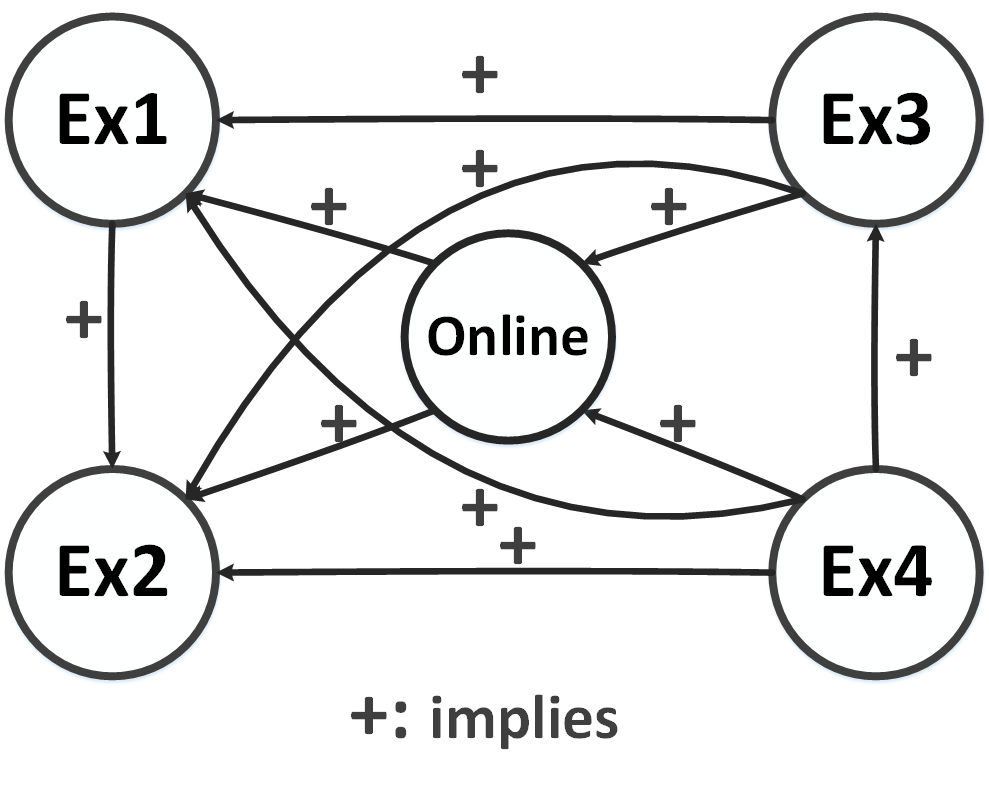
\includegraphics[scale=0.28]{figures/Fig8.png}}
	}}
      
      \caption{The implication relationships graph between existing observability 1, 2, 3, 4, and online observability where ``+" means ``implies".}
      \label{fig:7}
   \end{figure}
When I learned the four existing kinds of observability of \BCNs, I found that if we want to determine the initial state of a \BCN\ by first kind of observability, we need to guess the initial state of the \BCN\ and then check it by its corresponding input sequence. If the initial state we guess is right then we can determine the initial state of this \BCN. But if what we guess is incorrect, we need to guess the initial state again and use its corresponding input sequence to determine the initial state of this \BCN. We repeat this process untll we determine the initial state of this \BCN. But if we can not repeat this process, we can not determine the initial state of the \BCN\ too. Then I turned my gaze to the third observability, this kind of observability makes we can determine the initial state without presupposing the initial state. But I thought if we can determine the possible states set of the \BCN\ by observing the output at first, why do not we find corresponding input sequences for these possible states sets when we determine the initial state of \BCN? Compared with the existing third observability this method needs weaker preconditions of \BCNs\ for us to determine their initial state. Then I talked about this thinkness with my teacher, and we expand it into the original idea of the online observability of \BCNs. 

From the informal definition and formal definition of online observability, we can know that the necessary and sufficient condition of determine the initial state of \BCNs\ in real time is the online observability of \BCNs. With the online observability we can find the best way we like to determine the initial state of some biological systems which represented by \BCNs.
%==============================================================================================================